\documentclass{./../../Latex/teaching_slides}

\usepackage{venndiagram}
\usepackage{tikz}
\usepackage{pgfplots}
\usetikzlibrary{arrows.meta}

\begin{document}

\title{ECON 441 \\ \vspace{0.4em} \normalsize Introduction to Mathematical Economics}
\author{Div Bhagia}
\date{Lecture 6: Calculus}

%%%%%%%%%%%%%%
\begin{frame}[noframenumbering, plain]
\maketitle
\end{frame}


%%%%%%%%%%%%%%
\begin{frame}{Example}
Total cost: $C=C(Q)$ \\~\\
Marginal cost: $MC = C'(Q)$ \\~\\
Average cost:
$$ AC = \frac{C(Q)}{Q} $$ \\~\\
When is $ \frac{d AC}{d Q} $ positive?
\end{frame}


%%%%%%%%%%%%%%
\begin{frame}{Example}
Revenue: $R=f(Q)$ \\~\\
Output: $Q = g(L)$ \\~\\
How does revenue change due to a change in labor input $L$?
$$ \frac{d R}{d L} = \frac{d R}{d Q} \cdot \frac{d Q}{d L} $$ \\~\\
\end{frame}

%%%%%%%%%%%%%%
\begin{frame}{Exponential Functions}
The exponential or power function can be represented as:
$$
y=f(t)=b^{t} \quad(b>1)
$$
where $b$ denotes a fixed base of the exponent. \\
\vspace{1cm}
A more generalized version can be written as:
$$
y=a b^{c t}
$$
\end{frame}

%%%%%%%%%%%%%%
\begin{frame}{Natural Exponential Function}
Natural exponential function: Base is a special mathematical constant called Euler's number $e=2.71828...$

$$
y=a e^{r t}
$$ 
\vspace{1em}

\pause
Where did this number $e$ come from? \\~\\
It can be shown: $$
e \equiv \lim _{n \rightarrow \infty}\left(1+\frac{1}{n}\right)^{n}
$$
\end{frame}

%%%%%%%%%%%%%%
\begin{frame}{Natural Exponential Function}
Jacob Bernoulli discovered this constant in 1683 while studying a question about compound interest.
\end{frame}

%%%%%%%%%%%%%%
\begin{frame}{Logarithmic Function}
Since the exponential function is a monotonic function, its inverse exists. \\~\\
The inverse of the exponential function is called the log or logarithmic function. \\~\\
For the exponential function: 
\[ y=b^{t} \rightarrow log_b(y) = t  \]
For the natural exponential function:
\[y=e^{t} \rightarrow \log _{e} y =ln(y) \]
\end{frame}


\pgfplotsset{%
    width=10cm,
    height=8cm
}

%%%%%%%%%%%%%%
\begin{frame}{$y=exp(x)$}
\centering
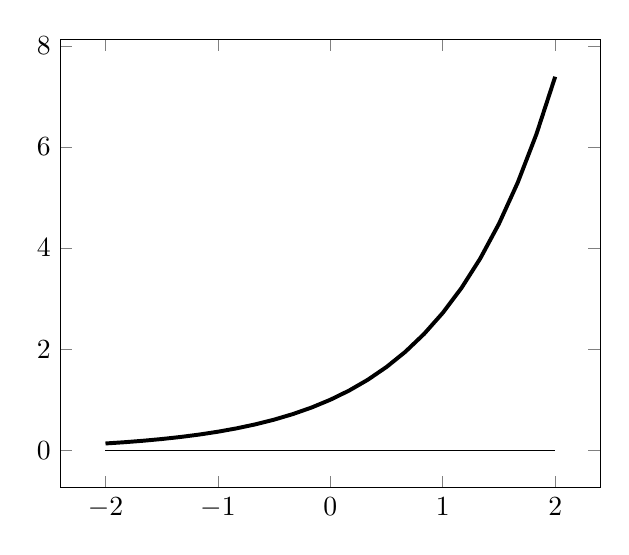
\begin{tikzpicture}
\begin{axis}[]
\addplot[color=black, line width=0.5mm, domain=-2:2] {exp(x)};
\addplot[domain=-2:2] {0};
\end{axis}
\end{tikzpicture} 
\end{frame}

%%%%%%%%%%%%%%
\begin{frame}{$y=ln(x)$}
\centering
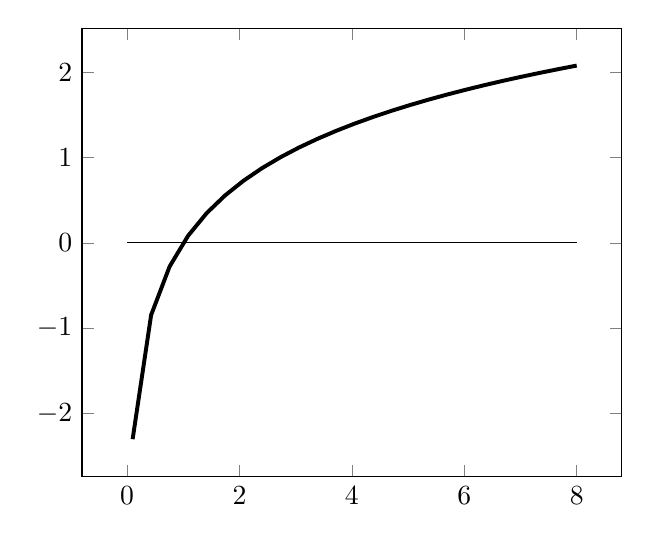
\begin{tikzpicture}
\begin{axis}[]
\addplot[color=black, line width=0.5mm, domain=0.1:8] {ln(x)};
\addplot[domain=0:8] {0};
\end{axis}
\end{tikzpicture} 
\end{frame}


%%%%%%%%%%%%%%
\begin{frame}{Rules for Logarithmic Functions}
\begin{witemize}
	\item $\ln (u v)=\ln u+\ln v$
	\item $\ln (u / v)=\ln u-\ln v$
	\item $\ln u^{a}=a \ln u$
\end{witemize}
\end{frame}

%%%%%%%%%%%%%%
\begin{frame}{Derivatives of Exponential Functions}
Derivative of the exponential function:
 $$y=e^{t} \quad \rightarrow \quad \frac{dy}{dt} = e^t$$
Using the chain rule: 
 $$y=e^{f(t)} \quad \rightarrow \quad \frac{dy}{dt} = f'(t) e^{f(t)}$$
 \end{frame}

 %%%%%%%%%%%%%%
 \begin{frame}{Derivatives of Logarithmic Functions}
Derivative of the log function:
 $$ \frac{d}{d t} \ln t =\frac{1}{t} $$
Using the chain rule: 
 $$ \frac{d}{d t} \ln f(t) =\frac{f'(t)}{f(t)} $$
\end{frame}

%%%%%%%%%%%%%%
\begin{frame}{Examples}
Find the derivatives for the following functions:\\
\begin{enumerate}
\item $y=e^t$
\item $y=\ln t$
\item $y=ae^{rt}$
\item $y=e^{-t}$
\item $y=\ln a t$
\item $y=\ln t^{c}$
\end{enumerate}
\end{frame}


%%%%%%%%%%%%%%
\begin{frame}{Partial Differentiation}

For a function of several variables:
$$
y=f\left(x_{1}, x_{2}, \cdots, x_{n}\right)
$$

If $x_1$ changes by $\Delta x_1$ but all other variables remain constant: 
$$
\frac{\Delta y}{\Delta x_{1}}=\frac{f\left(x_{1}+\Delta x_1, x_{2}, \cdots, x_{n}\right)-f\left(x_{1}, x_{2}, \cdots, x_{n}\right)}{\Delta x_{1}}
$$
Partial derivative of $y$ with respect to $x_i$:
$$
\frac{\partial y}{\partial x_{i}}= f_i = \lim _{\Delta x_{i} \rightarrow 0} \frac{\Delta y}{\Delta x_{i}}
$$
\end{frame}

%%%%%%%%%%%%%%
\begin{frame}{Partial Derivatives}
\centering
	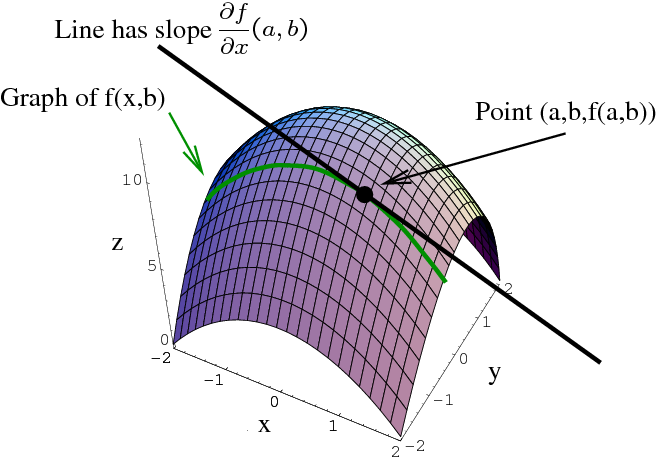
\includegraphics[scale=0.45]{3dpartial.png}
\end{frame}

%%%%%%%%%%%%%%
\begin{frame}{Gradient Vector}

Gradient: vector of all partial derivatives of a function

$$ \nabla f(x_1, x_2, \cdots, x_n) = [f_1, f_2, \cdots, f_n]' $$
\end{frame}

%%%%%%%%%%%%%%
\begin{frame}{Example}
	$$y=f\left(x_{1}, x_{2}\right)=3 x_{1}^{2}+x_{1} x_{2}+4 x_{2}^{2}$$
	
	$$\frac{\partial y}{ \partial x_{1}} = f_1 =  \hspace{5cm} $$
	
	$$\frac{\partial y}{ \partial x_{2}} = f_2 =  \hspace{5cm} $$

\end{frame}

%%%%%%%%%%%%%%
\begin{frame}{Example}
	$$y=f(u, v)=(u+4)(3 u+2 v)$$
	
	$$\frac{\partial y}{ \partial u} = f_u =  \hspace{5cm} $$
	
	$$\frac{\partial y}{ \partial v} = f_v =  \hspace{5cm} $$

\end{frame}

%%%%%%%%%%%%%%
\begin{frame}{Production Function}
$$ Q = A K^{\alpha} L^{1-\alpha} $$ \\~\\

Marginal product of capital (MPK):
	$$\frac{\partial Q}{ \partial K} = Q_K =  \hspace{5cm} $$

Marginal product of labor (MPL):
	$$\frac{\partial Q}{ \partial L} = Q_L =  \hspace{5cm} $$
\end{frame}

%%%%%%%%%%%%%%
\begin{frame}{Differentials}
%\vspace{1em}
Note that, 
$$
\Delta y \equiv\left[\frac{\Delta y}{\Delta x}\right] \Delta x
$$ \\~\\

Then for infinitesimal changes,
$$
d y \equiv\left[\frac{d y}{d x}\right] d x \quad \text {or} \quad d y=f^{\prime}(x) d x
$$ \\~\\

We will call $d y$ and $dx$ differentials of $y$ and $x$, respectively.
\end{frame}

%%%%%%%%%%%%%%
\begin{frame}{Derivative as a ratio}
	Given that, 
	$$
d y \equiv\left[\frac{d y}{d x}\right] d x \quad \text {or} \quad d y=f^{\prime}(x) d x
$$ \\~\\
We can think of $f'(x)$ as a ratio of two quantities $ dy $ and $dx$. 
 \end{frame}

%%%%%%%%%%%%%%
\begin{frame}{Elasticity}
An important quantity that economists love to calculate is the elasticity of a function. \\~\\
Elasticity is defined as:
\[ \varepsilon = \frac{\text{Percentage change in y}}{\text{Percentage change in x}} = \frac{dy/y}{dx/x} \] \\

We can calculate this as:
\[ \varepsilon = \frac{dy}{dx} \cdot \frac{x}{y} \]
\end{frame}

%%%%%%%%%%%%%%
\begin{frame}{Elasticity}
Elasticity: 
\[ \varepsilon = \frac{dy}{dx} \cdot \frac{x}{y} \]
\vspace{1cm}
\begin{itemize}
	\item $|\varepsilon|>1$, elastic
	\item $|\varepsilon|=1$, unit elasticity
	\item $|\varepsilon|<1$, inelastic
\end{itemize}
\end{frame}

%%%%%%%%%%%%%%
\begin{frame}{Example}
$$ C = a + bY $$
\end{frame}

%%%%%%%%%%%%%%
\begin{frame}{Total Differential}
For a function of $n$ variables \[y=f\left(x_{1}, x_{2}, \cdots, x_{n}\right)\]
Total differential:
\[
d f=\frac{\partial f}{\partial x_{1}} d x_{1}+\frac{\partial f}{\partial x_{2}} d x_{2}+\cdots+\frac{\partial f}{\partial x_{n}} d x_{n}=\sum_{i=1}^{n} f_{i} d x_{i}
\]

\vspace{1em}
\textit{I am using $\partial$ to differentiate partial derivatives from total derivatives. In particular, $$\left.\frac{\partial f}{\partial x_{i}} = \frac{d f}{d x_{i}} \right\vert_{\text{other variables are constant}} $$}
\end{frame}

%%%%%%%%%%%%%%
\begin{frame}{Total Differential}
Consider a savings function:
\[
S=S(Y, i)
\]
where $S$ is savings, $Y$ is national income, and $i$ is the interest rate. \\~\\
Total differential:
\[ 
d S=\frac{\partial S}{\partial Y} d Y+\frac{\partial S}{\partial i} d i
\]
\end{frame}

%%%%%%%%%%%%%%
\begin{frame}{Example}
$$ y = 5 x_1^2 + 3x_2 $$
\end{frame}


%%%%%%%%%%%%%%
\begin{frame}{Total Derivative}
Total differential:
\[
d f= f_1 d x_{1}+ f_2 d x_{2}+\cdots+f_n d x_{n}
\] \vspace{0.25em}

We can divide the total differential by $dx_1$ to get the \textit{total derivative} of $f$ with respect to $x_1$:
\[
\frac{d f}{dx_1} = f_1 + f_2 \cdot \frac{d x_{2}}{d x_{1}}+\cdots+f_n \cdot\frac{d x_{n}}{d x_{1}}
\]
\end{frame}

%%%%%%%%%%%%%%
\begin{frame}{Total Derivative}
Given the function 
\[ y = f(x_1, x_2) \]

We are interested in how $y$ changes with respect to $x_1$, but $x_2$ also depends of $x_1$
\[ x_2 = g(x_1) \]
We know that, 
\[ dy = f_1 dx_1 + f_2dx_2 \]

Dividing both sides by $dx_1$, 
\[ \frac{dy}{dx_1} =  f_1+f_2 \cdot g'(x_1) = \frac{\partial y}{\partial x_1} + \frac{\partial y}{\partial x_2} \cdot \frac{d x_2}{dx_1}  \]
\end{frame}

%%%%%%%%%%%%%%
\begin{frame}{A variation on the theme}
For a function
$$
y=f\left(x_{1}, x_{2}, w\right), \quad \quad x_{1}=g(w), x_{2}=h(w)
$$

\vspace{1cm}
The total derivative of $y$ is given by

$$
\frac{d y}{d w}=\frac{\partial f}{\partial x_{1}} \frac{d x_{1}}{d w}+\frac{\partial f}{\partial x_{2}} \frac{d x_{2}}{d w}+\frac{\partial f}{\partial w} 
$$
\end{frame}

%%%%%%%%%%%%%%
\begin{frame}{Example}
Let a production function be
$$
Q(t) = A(t) K(t)^{\alpha} L(t)^{1-\alpha} 
$$
where 

$$
K(t) = K_0 + at  \quad \quad L(t) = L_0 + bt
$$
\end{frame}


%%%%%%%%%%%%%%
\begin{frame}{Another variation on the theme}
If a function is given,
$$
y=f\left(x_{1}, x_{2}, u, v\right)
$$
with $x_{1}=g(u, v)$ and $x_{2}=h(u, v)$. \\~\\

Then,

\[\frac{d y}{d u}=\frac{\partial y}{\partial x_{1}} \frac{\partial x_{1}}{\partial u}+\frac{\partial y}{\partial x_{2}} \frac{\partial x_{2}}{\partial u}+\frac{\partial y}{\partial u}\]
\end{frame}

%%%%%%%%%%%%%%%
%\begin{frame}{Implicit Functions}
%Explicit function:
%$$y=f\left(x_{1}, x_{2}, \cdots, x_{n}\right)$$
%
%\vspace{1cm}
%Implicit function:
%\[F\left(y, x_{1}, x_{2}, \cdots, x_{n}\right)=0\]
%\end{frame}
%
%%%%%%%%%%%%%%%
%\begin{frame}{Example}
%Implicit function:
%\[ F(x,y)=y-3x^2 =0 \] \\ \vspace{1em}
%Corresponding explicit function:
%$$ y = f(x) = 3x^2 $$ \\ \vspace{1em}
%However, not all implicit functions have a corresponding explicit function. E.g. $F(x,y) = x^2 + y^2 -9=0$
%\end{frame}
%
%
%%%%%%%%%%%%%%%
%\begin{frame}{Implicit Function Theorem}
%Given,
%\[F\left(x, y \right)=0\]
%
%\vspace{1em}
%If the following conditions are met: \\ \vspace{0.5em}
%\begin{witemize}
%  \item $F_y$ and $F_x$ are continuous, and
%  \item At some point $(a,b)$, $F_y$ is non-zero  \\~\\
%\end{witemize}
%Then in a neighborhood around $(a,b)$, an implicit function exists. Moreover, this function is continuous and has continuous partial derivatives. 
%\end{frame}
%
%%%%%%%%%%%%%%%
%\begin{frame}{Derivatives of Implicit Functions}
%
%Total differentiating $F$, we have $d F=0$, or
%$$
%F_{y} d y+F_{1} d x_{1}+\cdots+F_{n} d x_{n}=0 
%$$
%
%\vspace{1em}
%Suppose that only $y$ and $x_{1}$ are allowed to vary:
%$$
%\frac{\partial y}{\partial x_{1}}=-\frac{F_{1}}{F_{y}} .
%$$
%
%\vspace{1em}
%In the simple case where the given equation is $F(y, x)=0$, the rule gives
%$$
%\frac{d y}{d x}=-\frac{F_{x}}{F_{y}} .
%$$
%\end{frame}
%
%%%%%%%%%%%%%%%
%\begin{frame}{Example}
%Given the following function, let's find $\partial y/\partial x$ and $\partial y/\partial z$. 
%$$ F(x,y,z) = x^3 z^2+y^3+4xyz = 0  $$
%\end{frame}
%
%%%%%%%%%%%%%%%
%\begin{frame}{Another Example}
%Estimate the following model for demand for fast food:
%$$ orders = \beta_0 + \beta_1 price + \beta_2 quality + \varepsilon   $$
%What is the interpretation of $\beta_1$?
%\end{frame}
%
%%%%%%%%%%%%%%%
%\begin{frame}{Another Example (cont.)}
%What if instead we estimate:
%$$ \ln(orders) = \beta_0 + \beta_1 \ln(price) + \beta_2 quality + \varepsilon   $$
%What is the interpretation of $\beta_1$?
%\end{frame}
%
%%%%%%%%%%%%%%%
%\begin{frame}{Another related example}
%Production function: 
%$$ Y = A L^{\alpha} K^\beta  $$ \vspace{0.5em}
%
%To estimate the elasticities from data:
%$$ \ln Y = \ln A + \alpha \ln L+ \beta \ln K + \varepsilon $$
%
%\end{frame}


%%%%%%%%%%%%%%
\begin{frame}{References and Homework}
References: Chapter 10 (notes are sufficient), Section 10.5, Section 7.4, Sections 8.1, 8.2, 8.4 \\~\\
 Homework problems: \\
  \begin{itemize}
  \normalsize
  	\item Ex 10.5: 1, 3, 7
    \item Ex 7.4 1 (a) (d), 2 (a) (b), 3, 5, 7;
    \item Ex 8.1: 1 (a), 4, 6; 
  	\item Ex 8.2: 3 (a), 4, 5, 6, 7 (b) (f); 
  	\item Ex 8.4: 2, 4; 
  	%\item Ex 8.5: 1, 2(d), 3 (a)
  	\end{itemize}
\end{frame}


\end{document}